\documentclass[letterpaper,11pt]{article}
%Document configuration
\usepackage{fullpage}
\usepackage[numbers]{natbib} 	%\citet{jon90} --> Jones et al. [21], \citep{jon90} --> [21]
\usepackage[capitalise]{cleveref}
\usepackage{amsthm}

%-------------- Personal commands begin --------------
\usepackage{dsfont,amssymb,amsfonts,enumitem}
\usepackage{graphicx,xcolor,tikz,comment}
	
%pgfplots configuration
\usepackage{pgfplots}
\pgfplotsset{compat=newest}
\pgfplotsset{ table/search path={TexImg/} }

\usepackage{caption}
\usepackage{subcaption}

\usepackage{algorithm,algpseudocode}
\renewcommand{\algorithmicrequire}{\textbf{Input:}}
\renewcommand{\algorithmicensure}{\textbf{Output:}}

\usepackage{mathtools}
\DeclarePairedDelimiter{\abs}{\lvert}{\rvert} %
\DeclarePairedDelimiter{\brk}{[}{]}
\DeclarePairedDelimiter{\crl}{\{}{\}}
\DeclarePairedDelimiter{\prn}{(}{)}


%Useful commands
\usepackage{minibox}
\newcommand{\anote}[1]{{\color{red}Alberto: #1}}		%to leave notes
\newcommand{\sbnote}[1]{{\color{blue}Sid: #1}}			
\newcommand{\sbedit}[1]{{\color{blue} #1}}				%to leave notes
\newcommand{\todo}[1]{{\color{green}TODO: #1}}		    %to leave notes

\newcommand{\E}{\mathbb{E}} 							%expectation
\newcommand{\Var}{\mathbb{V}\textnormal{ar}} 			%variance
\newcommand{\In}[1]{\mathds{1}_{\left\{ #1 \right\}}} 	%indicator
\newcommand{\R}{\mathbb{R}}								%reals
\newcommand{\N}{\mathbb{N}}								%naturals					
\renewcommand{\Pr}{\mathbb{P}}							%probability
\newcommand{\norm}[1]{\lvert\lvert#1\rvert\rvert}		%norm	
\newcommand{\card}[1]{\lvert#1\rvert}					%cardinal of a set
\newcommand{\ceil}[1]{\lceil#1\rceil}					%ceiling function
\newcommand{\Or}{O}
\newcommand{\defeq}{\coloneqq}							%symbol :=

%Additional commands
\newcommand{\calX}{\mathcal{X}}
\newcommand{\calP}{\mathcal{P}}							
\newcommand{\calQ}{\mathcal{Q}}							
\newcommand{\Bf}{B^+}									%forward ball
\newcommand{\Bb}{B^-}									%reverse ball
\newcommand{\Sf}{S^+}
\newcommand{\Sb}{S^-}
\newcommand{\Lf}{L^+}									%forward hub
\newcommand{\Lb}{L^-}									
\newcommand{\dist}{\mbox{dist}}							%distance
\newcommand{\pp}[1]{\langle#1\rangle}					%to denote pairs of nodes
\newcommand{\PE}{\mathcal{P}^E}							%efficient paths
\newcommand{\PB}{\mathcal{P}^B}							%shortest in G^B
\newcommand{\Pst}{\mathcal{P}_{s,t}}					%all paths s-t
\newcommand{\PS}{\mathcal{P}^*}							%shortest paths
\newcommand{\Gp}{\tilde G}								%pruned augmented graph
\newcommand{\Ep}{\tilde E}								%edges of pruned augmented
\newcommand{\Vp}{\tilde V}								%vertices of pruned augmented
\newcommand{\hc}{h_c}									%chd
\newcommand{\Lm}{L_{\mathrm{max}}}

%Theorems, lemmas, proofs, etc
\newtheorem{theorem}{Theorem}[section]
\newtheorem{proposition}[theorem]{Proposition}
\newtheorem{definition}[theorem]{Definition}
\newtheorem{lemma}[theorem]{Lemma}
\newtheorem{remark}[theorem]{Remark}
\let\oldproofname=\proofname
\renewcommand{\proofname}{{\sc\oldproofname}}

\renewcommand{\algorithmicrequire}{\textbf{Input:}}
\renewcommand{\algorithmicensure}{\textbf{Output:}}
			

\title{\vspace{-1cm} \bf Constrained Shortest Path \vspace{-1.3cm}}
\author{}
\begin{document}
\maketitle


\section{Average HD}

We relax the definition of HD in two ways.
First, a LSHS needs to be locally sparse just ``in average''.
Second, we forget the strong limitation of hitting $S_r(v,\calQ)$ and ask only for the existence of a multiscale LSHS.

\begin{definition}[Average LSHS]
Given $r>0$ and a system $\calQ$, a set $C\subseteq V$ is an average $(h,r)$-LSHS if it hits $\calQ_r$ and is locally sparse in average, i.e.,
\[
\frac{1}{\abs{V}}\sum_{v\in V} \abs{B_{2r}(v)\cap C} \leq h.
\]
\end{definition}

\begin{definition}[Average HD]
The system $\calQ$ has average HD $h$ if, for every $r>0$, there exists an average $(h,r)$-LSHS.
\anote{This can be further relaxed to only $r=2^i$. Furthermore, the value $h$ may vary across $r$.}
\end{definition}

\begin{theorem}\label{theo:preproc_avg}
If $\PS$ has average HD $h$, then we can obtain, in polynomial time, HL such that 
\[
\frac{1}{\abs{V}}\sum_{v\in V} \abs{\Lf(v)} \leq h'\log D \quad \text{ and }\quad
\frac{1}{\abs{V}}\sum_{v\in V} \abs{\Lb(v)} \leq h'\log D,
\]
where $h'=\Or(\Delta h\log (hn\Delta))$.
\end{theorem}
\begin{proof}
We only go over the preprocessing, since the construction does not change and the bound for the size easily follows. 
The objective is to obtain a set $C_i$ which is an average $(h',2^i)$-LSHS.
This is a minimum cost hitting set problem.
Indeed, we want to solve
\[
\min_{C\subseteq V} \sum_{v\in V}\abs{B_{2r}(v)\cap C}  \quad \text{ s.t. } \quad C \text{ hits } \PS_r.
\]
To see the equivalence, we assign to each node $u$ the cost $c(u)=\abs{\crl{v\in V: u\in B_{2r}(v)}}$.
Given a minimum cost hitting set problem with optimum value $\tau$, if the set system has VC-dimension $d$, the algorithm in \cite{vc_dim_hitting} finds a solution, in polynomial time, with cost at most $\Or(d\tau\log(d\tau))$.

By assumption, the minimum of the problem is at most $h\abs{V}$.
Now we do the same mapping as before, where the ground set is changed to $E$, hence the VC-dimension is 2 and now the minimum is at most $h\Delta\abs{V}$.
We apply the algorithm in \cite{vc_dim_hitting} and obtain a solution $C_i$ with cost at most $\Or(h\Delta\abs{V}\log(h\Delta\abs{V}))$.
We have obtained an average $(h',r)$-LSHS as desired.
\end{proof}

\begin{remark}
The algorithm in \cref{theo:preproc_avg} makes one call to the VC-dimension solver for each $C_i$.
On the other hand, the algorithm in \cite{highway2013} calls up to $n$ times the solver for each LSHS.
Finally, there is an extra $\log n$ factor in the approximation guarantee, but now the value of $h$ can be much smaller.
\end{remark}

The notion of average HD is more suitable for the CSP.
In particular, the existence of LSHS is guaranteed by the partial witness property, so now the preprocessing can be done agnostic of the value of $\beta$.

\begin{theorem}
If the average HD of $\PE$ is $h_c$, then we can obtain, in polynomial time, HL to answer queries with budget $b$ in average time $\Or(bh_c'\log D)$ and the space requirements are $\Or(nB\cdot Bh_c'\log D)$.
\end{theorem}

\section{Partial Witness Property}

An important notion is that, if efficient paths oscillate too much between free and tolled edges, then it is very unlikely to observe partial witnesses.
In Figure~\ref{fig:nosubpath} we present a graph with no $\frac{1}{2}$-partial witness.
Every edge has unit length, dash edges have zero cost and solid edges have unit cost.
The path $uvwx$ is efficient, but every subpath that is shortest has length one.
The example can be generalized by placing the graph side by side many times.
This shows that, for any constant $k$ we can find examples with no $\frac{1}{k}$-partial witnesses.


\begin{figure}
\caption{Example with unit cost and no subpath property}
\label{fig:nosubpath}
\centering
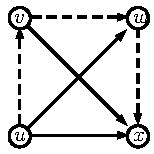
\includegraphics[scale=1.3]{TexImg/Nosubpath.pdf}
\end{figure}

\bibliographystyle{plainnat}
\bibliography{biblio}

\end{document}
